\chapter{Industry 4.0}
	\de{Digital manufacturing} is the evolution of manufacturing where an \textbf{integrated approach} is centered around a computer system. The evolution can be seen from purely mechanical machinery, to \textbf{CNC} \textit{computer numerical controlled} machines up to system of computer-controlled machines.	
	
	Digital manufacture goes in the framework of \de{Industry 4.0}, the fourth industrial revolution that politically \textit{started} in 2013 after Angela Merkel's request in 2011 at the \textit{Hannover Messe}. The final report of the \textit{Industrie 4.0} committee defines
	\begin{itemize}
		\item design principles;
		\item challenges;
		\item impacts
	\end{itemize}
	that industry 4.0 present.
	
	\paragraph{Objectives} The main goals of this fourth industrial revolution can be summarized as
	\begin{itemize}
		\item the political idea of re-shoring of added value in western countries after the 2008 economical crises and in order to re-establish independence from chines production;
		\item sustain the salaries of both workers and the middle-class;
		\item sustain the e-commerce;
		\item mass customization; this has been possible after a change of mentality in production: previously products were massively fabricated, stocked and only finally sold for a \textit{high} amount of time while now the time delay between production and final customer is reduced, improving the customization of the products;
		\item related to the previous point, a goal is to compress the life cycle of the product in order to make it available faster to the customers.
		
	\end{itemize}
	
	\paragraph{Design principles} The main design principle driving the industry 4.0 are:
	\begin{itemize}
		\item the \textbf{interoperability} exemplified by the \textit{Internet of Things} \de{IoT}, the \textit{Industrial IoT} \de{IIoT} and the \textit{Internet of People} \de{IoP}; this principle has the goal to increase the efficiency in communication between machines (\textit{things}) or persons (\textit{people}) with the goal to reduce the number of operators needed in a plant;
		\item the implementation of \textit{Cyber-Physical Systems} \de{CPS}, mechatronic machines allowed to communicate and exchange information in order to improve the production chain;
		\item the information transparency using \textbf{public} and \textbf{open protocols} that allows CPS to communicate with each-other using an unified \textit{language}. The realization of \textbf{digital twins} as a model that simulate the behaviour of a real cyber-physical system is also important in order to estimate how the whole components will interact together;
		\item the implementation of \textbf{self-support} and \textbf{in-line help} to guide the operators in troubleshooting errors that might occur during normal functioning;
		\item the \textbf{decision de-centralization} giving autonomy to CPS in order to make machines perform trivial choices according to a specific stratification and prioritization of the tasks, allowing humans to better focus on problems that need an high supervision.
	\end{itemize}
	
	This design principle can somehow related to \textit{the Yardstick of Automation}, an article published in 1962 by \textit{Amber\&Amber} that relates the order of automation by evaluating the human attributes that machines can substitute; such order are reported in table \ref{tab:ind:amber}. At this stage, with the industry 4.0, we consider industries between order 4 to 6 of that table.
	
	\begin{table}[bt]
		\centering
		\tabrule
		\caption{order nd related human attribute substituted (with example) according to "the Yardstick of Automation" article.} \label{tab:ind:amber}\vspace{2mm}
		\begin{tabular} { c c p{10cm} }
			Order & Human Attribute &  Example \\ \hline
			0 & none & manual tools \\
			1 & energy & powered machines and tools \\
			2 & dexterity & single-cycle automatics (\textit{dexterity} means \textit{self-feeding} in a sense of repeatable system) \\
			3 & diligence & repeats cycle, open-loop control; ability to perform all the action with the same accuracy \\
			4 & judgment & closed loop, numerical controls, self-measuring systems \\
			5 & evaluation & computer control, model of process required for automation \\
			6 & learning & limited self-programming and some artificial intelligence \\
			7 & reasoning & inductive reasoning (cause $\rightarrow$ effects) \\
			8 & creativity & performing original designs unaided \\
			9 & dominance & machine is a master
			
		\end{tabular}	
		
		\vspace{2mm}
		\tabrule
	\end{table}
	
	\paragraph{Challenges} At this stage the main challenges of industry 4.0 are:
	\begin{itemize}
		\item cybersecurity: cyber-physical systems are \textit{high-tech} equipment that has the weakness of being hacked with so the possibility of high damages to production and operators;
		\item reliability and resiliency of the communication \textit{machine-to-machine} \textbf{M2M} mainly determined by the bandwidth of communication but most importantly it's latency;
		\item system should be design with a drop-in, plug-in approach on existing processes; plants cannot be re-invented from scratch in order to introduce a new machine, but all the pieces should be able to work together following the same unified protocols and standards;
		\item the protection of the intellectual property (that's put in danger with the high frequency of exchanging digital files);
		\item the reluctancy of plant owner to change the way industry processes are made and the need of re-train operators;
		\item the initial loss of labor that will be in the years reconverted into a \textit{higher order} operators.
	\end{itemize}
	
	\paragraph{Impacts} The main impacts provided by industry 4.0 can be summarized in:
	\begin{itemize}
		\item \textit{servitization} as the passage from selling goods to selling services to people;
		\item the productivity and its resilience;
		\item safety for human operators;
		\item integrated design of product and process (the two things now will go together and shouldn't be consider as separate);
		\item the cos structure in terms of money allocation in the production process;
		\item the socio-economical factors;
		\item the ability to have a high number of data to analyse and process.
	\end{itemize}
	
\section*{Digital manufacturing and industry 4.0} 
	Regarding industry 4.0 and digital manufacturing some core enable technology are common such the M2M connectivity between cyber-physical system, the connectivity layer provided by the industry internet of things, the additive manufacturing as the dematerialization of the design and the machine learning/artificial intelligence to make autonomous decision possible.
	
	\paragraph{CPSs} Cyber-physical systems are mechatronic system, so mechanisms whose actuators are controlled by a computer system based on output from sensors and logics provided by algorithms. Digital manufacturing enables CPSs must be IoT-connected in order to provide the plant controller with information its own status and accept incoming tasks. \\
	The industrial internet of things has to support communication (M2M) between a number of CPSs that can be theoretically huge. In this sense \de{IP protocols} standard have been created allowing $4.3\cdot 10^9$ addresses for \texttt{IPv4} version and more recently \texttt{IPv6} allowing $3.4\cdot 10^{38}$ unique addresses.
	
	\subsection*{Networking model}
		According to the internet model, data can be exchanged between machines by creating a networking stack where the package is composed by 4 different layers stacked (as shown in figure \ref{fig:ind:netstack}).
		\begin{SCfigure}[2][b]
			\centering 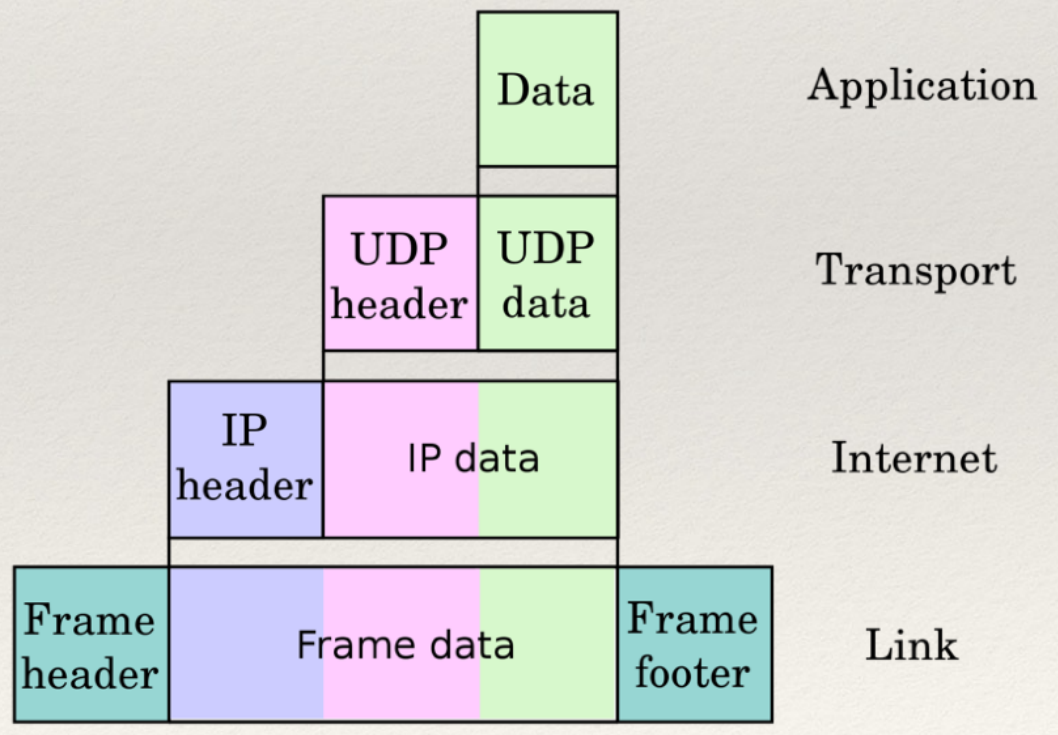
\includegraphics[width=6cm]{net-stack}
			\caption{4 layers and related package constitution used for communication using internet protocols.} \label{fig:ind:netstack}
		\end{SCfigure}
		Such layers are:
		\begin{itemize}
			\item[\texttt{L1})] link layer made by the physical carrier standard (such Ethernet cable or WiFi) and it's protocol (\texttt{MAC}, \texttt{813.11}, \texttt{ARP}...) that explains \textit{how} data are transmitted;
			\item[\texttt{L2})] internet (network) layer made by the addressing protocols (such \texttt{IPv4}, \texttt{IPv6} or \texttt{ICMP}) in order to properly address packages of information;
			\item[\texttt{L3})] transport layer (\texttt{TCP}, \texttt{UDP} protocols) that manages the connection between nodes in the network;
			\item[\texttt{L4})] application layer (such \texttt{HTTP}, \texttt{FTP}, \texttt{IMAP}, \texttt{LDAP} standards) that describes and contains encoded data.
		\end{itemize}
	
		The industrial internet of things must support communications between cyber-physical systems with a M2M communication; for the first layer \texttt{L1}, the link should be \textit{as fast as possible} in order to have a low latency and for this reason the new 5G protocol seems promising. Regarding instead the application layer \texttt{L4} protocols we can use the  more verbose and complex standard such \texttt{REST} or more lightweight ones (such \texttt{MQTT}, \texttt{ZeroMQ}, \texttt{AMQP} and \texttt{OPC-UA}).
	
		\paragraph{REST and HTTP overhead} The REST (\textit{REpresentational State Transfer}) is a protocol extended from HTTP and is characterized by a verbose (large) overhead, a complex syntax and by a connection $n$ machine to 1 server. The communication starts by sending 3 first packages for a hand-shake communication synchronization (no information are exchanged at this point) and only after this operation data are exchanged between one machine and the server. The headers of this communication is large: considering in fact that the simplest request phrase requires 14 bytes, the associated full request stack is made by 437 bytes (need of bigger bandwidth) and the number of packages sent back-and-forth between machine and server is \textit{high}, resulting in higher latency.
		
		The combination of handshaking protocols and verbose frame headers/footers allows to have a reliable and robust connection with a needed increase of bandwidth and with an increased latency; for this reason more \textit{machined based} protocols have been implemented in order to reduce latency while exchanging information between server and machines with the draw-back of reducing the number of packages sent resulting in less synchronization and confirmation (for example of package delivered).
	
		In IoP messages are frequently \textit{heavy} and seldom and the robustness of the HTTP protocol allows to better adapt the information exchanged between machines using different web servers or browsers. On the other hand IoT requires smaller messages sent with high frequency and so standard are enforced to minimize possible sources of unexpected conditions while still maintaining low latency.
		
		In IIoT messages also should follow routes more complex than $n$-to-1 ($n$ clients to 1 server) and so we need to minimize the overhead and support flexible topologies of the network infrastructure. A way to perform this operation is by using \textbf{message queuing protocols} (such \texttt{MQTT}, \texttt{ZeroMQ}) where clients can be both \textbf{publishers} and/or \textbf{subscribers} of the information; all this communication system is handled by the so called \textbf{broker}.\\
		The idea behind such type of communication is that clients that join a broker as publisher can send information to this intermediate server that immediately notifies all the subscribed machined with the information provided.
	
	
	
	
	
	
	
	
	
	
	
	
	
	
	
	